%% LaTeX-Beamer template for KIT design
%% by Erik Burger, Christian Hammer
%% title picture by Klaus Krogmann
%%
%% version 2.1
%%
%% mostly compatible to KIT corporate design v2.0
%% http://intranet.kit.edu/gestaltungsrichtlinien.php
%%
%% Problems, bugs and comments to
%% burger@kit.edu

\documentclass[18pt]{beamer}
\usepackage[utf8x]{inputenc}
\usepackage{units}
\usepackage{booktabs}

%% CUSTOM
\usepackage{amsmath}
\usepackage{algpseudocode}

%% Definitions
\DeclareMathOperator{\div2}{div}
\renewcommand{\algorithmicrequire}{\textbf{Input:}}
\renewcommand{\algorithmicensure}{\textbf{Output:}}
\algnewcommand\algorithmicto{\textbf{to}}
\algrenewtext{For}[3]{\algorithmicfor\ $#1 \gets #2$ \algorithmicto\ $#3$ \algorithmicdo}
\algnewcommand\algorithmicod{\textbf{od}}
\algrenewtext{EndWhile}{\algorithmicod}
\algrenewtext{EndFor}{\algorithmicod}
%\AtBeginSection[]{%
%\begin{frame}<beamer> % do nothing in handouts
%    \frametitle{Überblick}
%    \tableofcontents[sectionstyle=show/shaded,
%    subsectionstyle=show/show/hide]
%\end{frame}
%}
%\AtBeginSubsection[]{%
%\begin{frame}<beamer> % do nothing in handouts
%    \frametitle{Überblick}
%    \tableofcontents[sectionstyle=show/shaded,
%    subsectionstyle=show/shaded/hide]
%\end{frame}
%}

%% SLIDE FORMAT

% use 'beamerthemekit' for standard 4:3 ratio
% for widescreen slides (16:9), use 'beamerthemekitwide'

\usepackage{templates/beamerthemekit}
%\usepackage{templates/beamerthemekitwide}

 %% TITLE PICTURE

 % if a custom picture is to be used on the title page, copy it into the 'logos'
 % directory, in the line below, replace 'mypicture' with the 
 % filename (without extension) and uncomment the following line
 % (picture proportions: 63 : 20 for standard, 169 : 40 for wide
 % *.eps format if you use latex+dvips+ps2pdf, 
 % *.jpg/*.png/*.pdf if you use pdflatex)


 \titleimage{banner}
 
 
%% Define some colors:
\definecolor{darkblue}{rgb}{0,0,.5}
\definecolor{darkgreen}{rgb}{0,.5,0}

 %% TITLE LOGO

 % for a custom logo on the front page, copy your file into the 'logos'
 % directory, insert the filename in the line below and uncomment it

\titlelogo{logo_150x150}
 
 % (*.eps format if you use latex+dvips+ps2pdf,
 % *.jpg/*.png/*.pdf if you use pdflatex)
 
 %% TikZ INTEGRATION
 
 % use these packages for PCM symbols and UML classes
 % \usepackage{templates/tikzkit}
 % \usepackage{templates/tikzuml}
 
 % the presentation starts here
 
\author{Dominik Muth - dominik.muth@student.kit.edu}
\institute{Institut f\"ur Informatik}


\title[Tutorium 3]{GBI Tutorium Nr. 32}
\subtitle{Tutorium 3}
\date{7. November 2012}

% Bibliography



\begin{document}

	%title page
	\begin{frame}
		\titlepage
	\end{frame}

	%table of contents
	\begin{frame}{Outline/Gliederung}
		\tableofcontents
	\end{frame}
	
	
	\section{Übungsblatt 3}
	\begin{frame} {Übungsblatt 3}
		\begin{block} {Aufgabe 3.x}
			Aufgabe
		\end{block}
		\begin{overprint}
			$M$ sei die Menge aller Menschen.
			\onslide<2> $\forall x \in M: \exists_1 y\in M:B(x,y)$ ?
			\onslide<3-> \color{red} $\forall x \in M: \exists_1 y\in M:B(x,y)$!\\
			
		\end{overprint}
		\begin{overprint}
			\onslide<4> $\forall x \in M: \exists y \in M: B(x,y)$
			\onslide<5> $\forall x \in M: \exists y \in M: B(x,y)\land \forall z \in  M \! \setminus \! y: \lnot B(x,z)$
			\onslide<6> \color{darkgreen}$\forall x \in M: \exists y \in M: B(x,y)\land \forall z \in  M \! \setminus \! y: \lnot B(x,z)$
		\end{overprint}
	
	\end{frame}	
		
	
	\section{Wiederholung} 
	\begin{frame} {Wiederholung}
		\begin{itemize}
			\item $A^*$ ist eine formale Sprache! 
			\only<2-> {\color{darkgreen}$\surd$}\\
			\color{black}
		\end{itemize}
	\end{frame}
	
	
	



		
	\begin{frame} {EOF}
		\begin{center}
			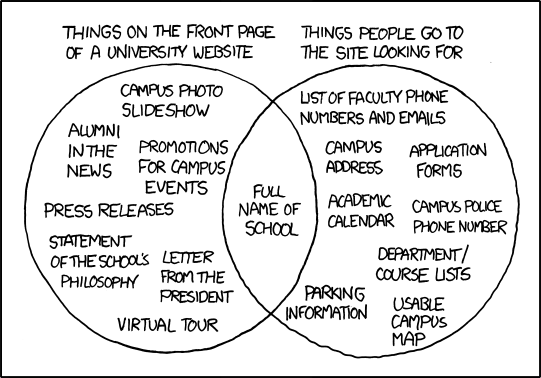
\includegraphics[scale=0.5]{graphics/02/eof2.png}\\
			\tiny $source: http://imgs.xkcd.com/comics/university_website.png$
		\end{center}
	\end{frame}

\end{document}
